\documentclass{standalone}
\usepackage{tikz}
\usetikzlibrary{patterns, positioning}


\begin{document}
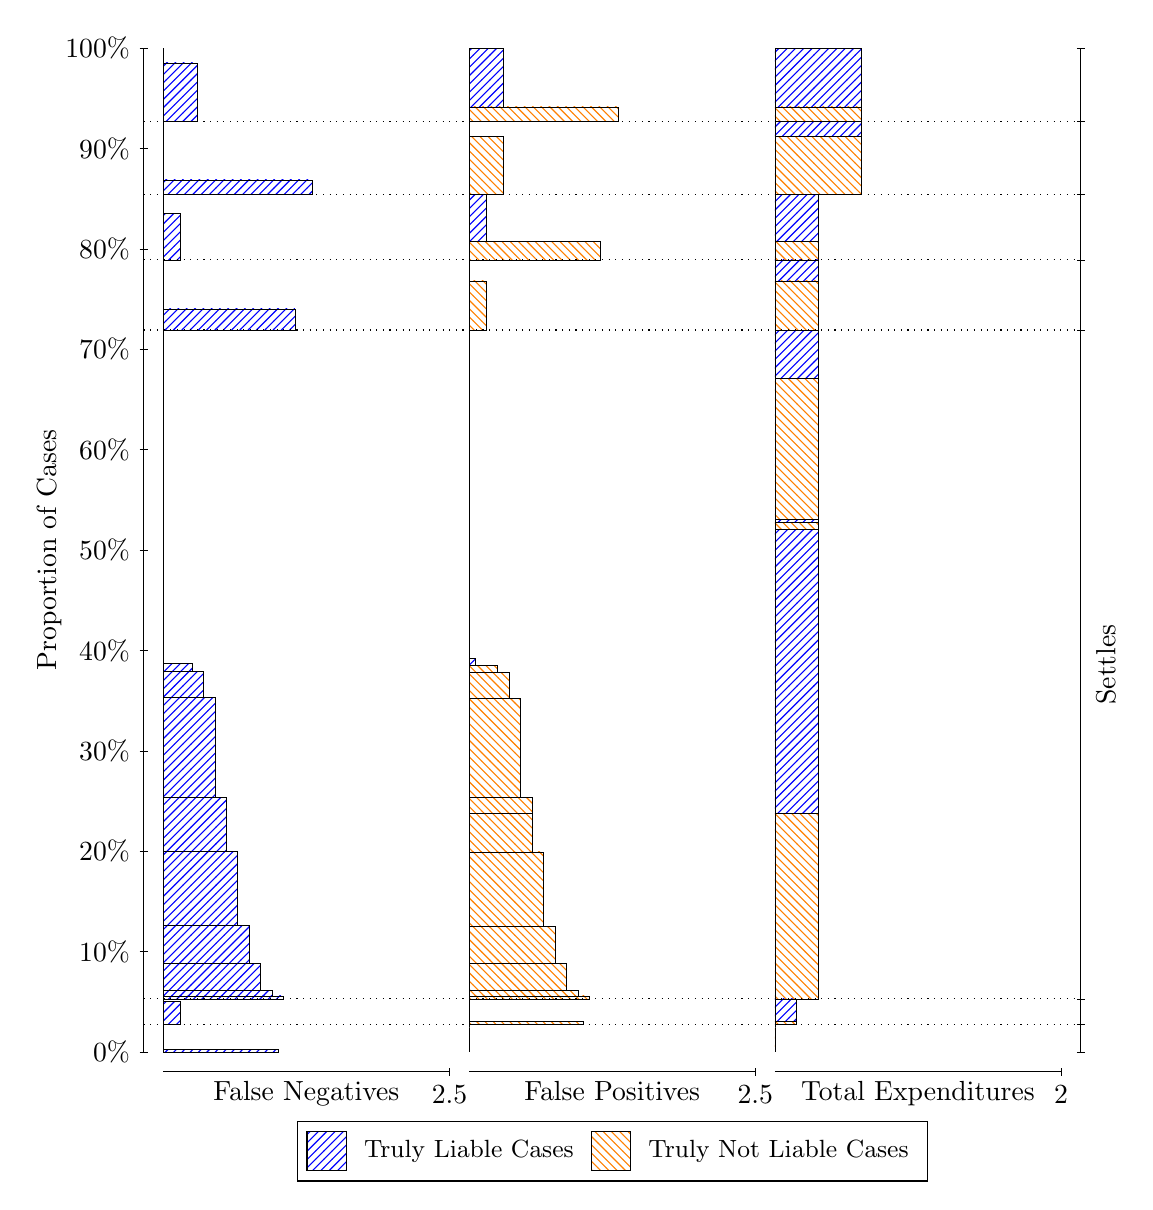
\begin{tikzpicture}
\draw[black, very thin] (1.5,1.75) -- (1.5,14.5);
\node[rotate=90, text=black, anchor=center] at (0.3, 8.125) {Proportion of Cases};
\draw[black, very thin] (1.45,1.75) -- (1.55,1.75);
\node[text=black, anchor=east] at (1.45, 1.75) {0\%};
\draw[black, very thin] (1.45,3.025) -- (1.55,3.025);
\node[text=black, anchor=east] at (1.45, 3.025) {10\%};
\draw[black, very thin] (1.45,4.3) -- (1.55,4.3);
\node[text=black, anchor=east] at (1.45, 4.3) {20\%};
\draw[black, very thin] (1.45,5.575) -- (1.55,5.575);
\node[text=black, anchor=east] at (1.45, 5.575) {30\%};
\draw[black, very thin] (1.45,6.85) -- (1.55,6.85);
\node[text=black, anchor=east] at (1.45, 6.85) {40\%};
\draw[black, very thin] (1.45,8.125) -- (1.55,8.125);
\node[text=black, anchor=east] at (1.45, 8.125) {50\%};
\draw[black, very thin] (1.45,9.4) -- (1.55,9.4);
\node[text=black, anchor=east] at (1.45, 9.4) {60\%};
\draw[black, very thin] (1.45,10.675) -- (1.55,10.675);
\node[text=black, anchor=east] at (1.45, 10.675) {70\%};
\draw[black, very thin] (1.45,11.95) -- (1.55,11.95);
\node[text=black, anchor=east] at (1.45, 11.95) {80\%};
\draw[black, very thin] (1.45,13.225) -- (1.55,13.225);
\node[text=black, anchor=east] at (1.45, 13.225) {90\%};
\draw[black, very thin] (1.45,14.5) -- (1.55,14.5);
\node[text=black, anchor=east] at (1.45, 14.5) {100\%};

\draw[black, very thin] (13.4,1.75) -- (13.4,14.5);
\draw[black, very thin] (13.35,1.75) -- (13.45,1.75);
\node[anchor=west] at (13.35, 1.75) {};
\draw[black, very thin] (13.35,2.0996) -- (13.45,2.0996);
\node[anchor=west] at (13.35, 2.0996) {};
\draw[black, very thin] (13.35,2.4243) -- (13.45,2.4243);
\node[anchor=west] at (13.35, 2.4243) {};
\draw[black, very thin] (13.35,10.919) -- (13.45,10.919);
\node[anchor=west] at (13.35, 10.919) {};
\draw[black, very thin] (13.35,11.809) -- (13.45,11.809);
\node[anchor=west] at (13.35, 11.809) {};
\draw[black, very thin] (13.35,12.637) -- (13.45,12.637);
\node[anchor=west] at (13.35, 12.637) {};
\draw[black, very thin] (13.35,13.564) -- (13.45,13.564);
\node[anchor=west] at (13.35, 13.564) {};
\draw[black, very thin] (13.35,14.5) -- (13.45,14.5);
\node[anchor=west] at (13.35, 14.5) {};

\draw[black, very thin, pattern color=blue, pattern=north east lines] (1.75,1.75) rectangle (3.2033,1.7868);
\draw[black, very thin, pattern color=orange, pattern=north west lines] (1.75,1.7868) rectangle (1.75,2.0996);
\draw[black, very thin, pattern color=blue, pattern=north east lines] (1.75,2.0996) rectangle (1.968,2.3903);
\draw[black, very thin, pattern color=orange, pattern=north west lines] (1.75,2.3903) rectangle (1.75,2.4243);
\draw[black, very thin, pattern color=blue, pattern=north east lines] (1.75,2.4243) rectangle (3.276,2.4618);
\draw[black, very thin, pattern color=blue, pattern=north east lines] (1.75,2.4618) rectangle (3.1307,2.5366);
\draw[black, very thin, pattern color=blue, pattern=north east lines] (1.75,2.5366) rectangle (2.9853,2.8759);
\draw[black, very thin, pattern color=blue, pattern=north east lines] (1.75,2.8759) rectangle (2.84,3.3559);
\draw[black, very thin, pattern color=blue, pattern=north east lines] (1.75,3.3559) rectangle (2.6947,4.3013);
\draw[black, very thin, pattern color=blue, pattern=north east lines] (1.75,4.3013) rectangle (2.5493,4.9869);
\draw[black, very thin, pattern color=blue, pattern=north east lines] (1.75,4.9869) rectangle (2.404,6.254);
\draw[black, very thin, pattern color=blue, pattern=north east lines] (1.75,6.254) rectangle (2.2587,6.5873);
\draw[black, very thin, pattern color=blue, pattern=north east lines] (1.75,6.5873) rectangle (2.1133,6.6801);
\draw[black, very thin, pattern color=orange, pattern=north west lines] (1.75,6.6801) rectangle (1.75,10.919);
\draw[black, very thin, pattern color=blue, pattern=north east lines] (1.75,10.919) rectangle (3.4213,11.186);
\draw[black, very thin, pattern color=orange, pattern=north west lines] (1.75,11.186) rectangle (1.75,11.809);
\draw[black, very thin, pattern color=blue, pattern=north east lines] (1.75,11.809) rectangle (1.968,12.397);
\draw[black, very thin, pattern color=orange, pattern=north west lines] (1.75,12.397) rectangle (1.75,12.637);
\draw[black, very thin, pattern color=blue, pattern=north east lines] (1.75,12.637) rectangle (3.6393,12.825);
\draw[black, very thin, pattern color=orange, pattern=north west lines] (1.75,12.825) rectangle (1.75,13.564);
\draw[black, very thin, pattern color=blue, pattern=north east lines] (1.75,13.564) rectangle (2.186,14.312);
\draw[black, very thin, pattern color=orange, pattern=north west lines] (1.75,14.312) rectangle (1.75,14.5);
\draw[black, very thin, pattern color=orange, pattern=north west lines] (5.6333,1.75) rectangle (5.6333,2.0629);
\draw[black, very thin, pattern color=blue, pattern=north east lines] (5.6333,2.0629) rectangle (5.6333,2.0996);
\draw[black, very thin, pattern color=orange, pattern=north west lines] (5.6333,2.0996) rectangle (7.0867,2.1337);
\draw[black, very thin, pattern color=blue, pattern=north east lines] (5.6333,2.1337) rectangle (5.6333,2.4243);
\draw[black, very thin, pattern color=orange, pattern=north west lines] (5.6333,2.4243) rectangle (7.1593,2.461);
\draw[black, very thin, pattern color=orange, pattern=north west lines] (5.6333,2.461) rectangle (7.014,2.5365);
\draw[black, very thin, pattern color=orange, pattern=north west lines] (5.6333,2.5365) rectangle (6.8687,2.8794);
\draw[black, very thin, pattern color=orange, pattern=north west lines] (5.6333,2.8794) rectangle (6.7233,3.3485);
\draw[black, very thin, pattern color=orange, pattern=north west lines] (5.6333,3.3485) rectangle (6.578,4.2912);
\draw[black, very thin, pattern color=orange, pattern=north west lines] (5.6333,4.2912) rectangle (6.4327,4.7767);
\draw[black, very thin, pattern color=orange, pattern=north west lines] (5.6333,4.7767) rectangle (6.4327,4.982);
\draw[black, very thin, pattern color=orange, pattern=north west lines] (5.6333,4.982) rectangle (6.2873,6.238);
\draw[black, very thin, pattern color=orange, pattern=north west lines] (5.6333,6.238) rectangle (6.142,6.5662);
\draw[black, very thin, pattern color=orange, pattern=north west lines] (5.6333,6.5662) rectangle (5.9967,6.6632);
\draw[black, very thin, pattern color=blue, pattern=north east lines] (5.6333,6.6632) rectangle (5.706,6.756);
\draw[black, very thin, pattern color=blue, pattern=north east lines] (5.6333,6.756) rectangle (5.6333,10.919);
\draw[black, very thin, pattern color=orange, pattern=north west lines] (5.6333,10.919) rectangle (5.8513,11.542);
\draw[black, very thin, pattern color=blue, pattern=north east lines] (5.6333,11.542) rectangle (5.6333,11.809);
\draw[black, very thin, pattern color=orange, pattern=north west lines] (5.6333,11.809) rectangle (7.3047,12.048);
\draw[black, very thin, pattern color=blue, pattern=north east lines] (5.6333,12.048) rectangle (5.8513,12.637);
\draw[black, very thin, pattern color=orange, pattern=north west lines] (5.6333,12.637) rectangle (6.0693,13.375);
\draw[black, very thin, pattern color=blue, pattern=north east lines] (5.6333,13.375) rectangle (5.6333,13.564);
\draw[black, very thin, pattern color=orange, pattern=north west lines] (5.6333,13.564) rectangle (7.5227,13.752);
\draw[black, very thin, pattern color=blue, pattern=north east lines] (5.6333,13.752) rectangle (6.0693,14.5);
\draw[black, very thin, pattern color=orange, pattern=north west lines] (9.5167,1.75) rectangle (9.5167,2.0629);
\draw[black, very thin, pattern color=blue, pattern=north east lines] (9.5167,2.0629) rectangle (9.5167,2.0996);
\draw[black, very thin, pattern color=orange, pattern=north west lines] (9.5167,2.0996) rectangle (9.7892,2.1337);
\draw[black, very thin, pattern color=blue, pattern=north east lines] (9.5167,2.1337) rectangle (9.7892,2.4243);
\draw[black, very thin, pattern color=orange, pattern=north west lines] (9.5167,2.4243) rectangle (10.062,4.7767);
\draw[black, very thin, pattern color=blue, pattern=north east lines] (9.5167,4.7767) rectangle (10.062,8.3821);
\draw[black, very thin, pattern color=orange, pattern=north west lines] (9.5167,8.3821) rectangle (10.062,8.479);
\draw[black, very thin, pattern color=blue, pattern=north east lines] (9.5167,8.479) rectangle (10.062,8.5165);
\draw[black, very thin, pattern color=orange, pattern=north west lines] (9.5167,8.5165) rectangle (10.062,10.306);
\draw[black, very thin, pattern color=blue, pattern=north east lines] (9.5167,10.306) rectangle (10.062,10.919);
\draw[black, very thin, pattern color=orange, pattern=north west lines] (9.5167,10.919) rectangle (10.062,11.542);
\draw[black, very thin, pattern color=blue, pattern=north east lines] (9.5167,11.542) rectangle (10.062,11.809);
\draw[black, very thin, pattern color=orange, pattern=north west lines] (9.5167,11.809) rectangle (10.062,12.048);
\draw[black, very thin, pattern color=blue, pattern=north east lines] (9.5167,12.048) rectangle (10.062,12.637);
\draw[black, very thin, pattern color=orange, pattern=north west lines] (9.5167,12.637) rectangle (10.607,13.375);
\draw[black, very thin, pattern color=blue, pattern=north east lines] (9.5167,13.375) rectangle (10.607,13.564);
\draw[black, very thin, pattern color=orange, pattern=north west lines] (9.5167,13.564) rectangle (10.607,13.752);
\draw[black, very thin, pattern color=blue, pattern=north east lines] (9.5167,13.752) rectangle (10.607,14.5);
\draw[black, dotted] (1.5,2.0996) -- (13.4,2.0996);
\draw[black, dotted] (1.5,2.4243) -- (13.4,2.4243);
\draw[black, dotted] (1.5,10.919) -- (13.4,10.919);
\draw[black, dotted] (1.5,11.809) -- (13.4,11.809);
\draw[black, dotted] (1.5,12.637) -- (13.4,12.637);
\draw[black, dotted] (1.5,13.564) -- (13.4,13.564);
\draw[black, very thin] (1.75,1.5) -- (5.3833,1.5);
\node[text=black, anchor=north] at (3.5667, 1.5) {False Negatives};
\draw[black, very thin] (5.3833,1.45) -- (5.3833,1.55);
\node[text=black, anchor=north] at (5.3833, 1.45) {2.5};

\draw[black, very thin] (5.6333,1.5) -- (9.2667,1.5);
\node[text=black, anchor=north] at (7.45, 1.5) {False Positives};
\draw[black, very thin] (9.2667,1.45) -- (9.2667,1.55);
\node[text=black, anchor=north] at (9.2667, 1.45) {2.5};

\draw[black, very thin] (9.5167,1.5) -- (13.15,1.5);
\node[text=black, anchor=north] at (11.333, 1.5) {Total Expenditures};
\draw[black, very thin] (13.15,1.45) -- (13.15,1.55);
\node[text=black, anchor=north] at (13.15, 1.45) {2};



\node[text=black, centered, rotate=90] at (13.72, 6.6716) {Settles};





\draw (7.449999999999999,1.5) node[draw=none] (baseCoordinate) {};
\begin{scope}[align=center]
        \matrix[scale=0.5, draw=black, below=0.5cm of baseCoordinate, nodes={draw}, column sep=0.1cm]{
            \node[rectangle, draw, minimum width=0.5cm, minimum height=0.5cm, pattern color=blue, pattern=north east lines] {}; &
            \node[draw=none, font=\small, text=black] (B) {Truly Liable Cases}; &
            \node[rectangle, draw, minimum width=0.5cm, minimum height=0.5cm, pattern color=orange, pattern=north west lines] {}; &
            \node[draw=none, font=\small, text=black] (B) {Truly Not Liable Cases}; \\
            };
\end{scope}

\end{tikzpicture}
\end{document}